\documentclass{article}

\usepackage{circuitikz}

\begin{document}

% INT_AY21_L30_Fig01_Series_parallel.png

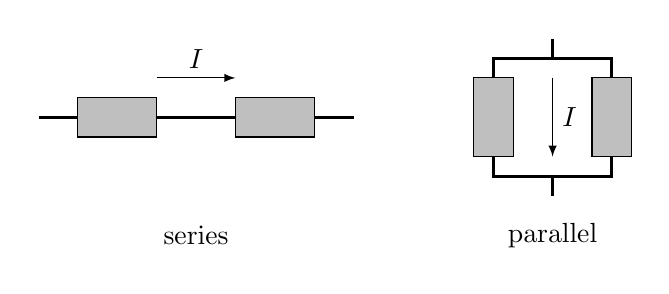
\begin{tikzpicture}[> = latex]
\matrix[column sep = 1.5 cm]{

	% Circuit elements
	
	\begin{scope}[gray!50, draw = black]
	
		\filldraw (-1.5, -0.25) rectangle (-0.5, 0.25);
		\filldraw (0.5, -0.25) rectangle (1.5, 0.25);
	
	\end{scope}
	
	% Wires
	
	\begin{scope}[very thick]
	
		\draw (-2, 0) -- (-1.5, 0);
		\draw (-0.5, 0) -- (0.5, 0);
		\draw (1.5, 0) -- (2, 0);
	
	\end{scope}
	
	% Current flow
	
	\draw [->] (-0.5, 0.5) -- node [above] {$I$} (0.5, 0.5);
	
	% Label
	
	\node at (0, -1.5) {series};

&

	% Circuit elements
	
	\begin{scope}[gray!50, draw = black]

		\filldraw (-1, -0.5) rectangle (-0.5, 0.5);
		\filldraw (1, -0.5) rectangle (0.5, 0.5);
	
	\end{scope}
	
	% Wires
	
	\begin{scope}[very thick]
		
		\draw (0, 0.75) -- (0, 1);
		\draw (-0.75, 0.5) -- (-0.75, 0.75) -- (0.75, 0.75) -- (0.75, 0.5);
		\draw (-0.75, -0.5) -- (-0.75, -0.75) -- (0.75, -0.75) -- (0.75, -0.5);
		\draw (0, -0.75) -- (0, -1);
	
	\end{scope}
	
	% Current flow
	
	\draw [->] (0, 0.5) -- node [right] {$I$} (0, -0.5);
	
	% Label
	
	\node at (0, -1.5) {parallel};

\\	
};

\end{tikzpicture}

\vspace{1em}

% INT_AY21_L30_Fig02_Missing_curr_volt.png

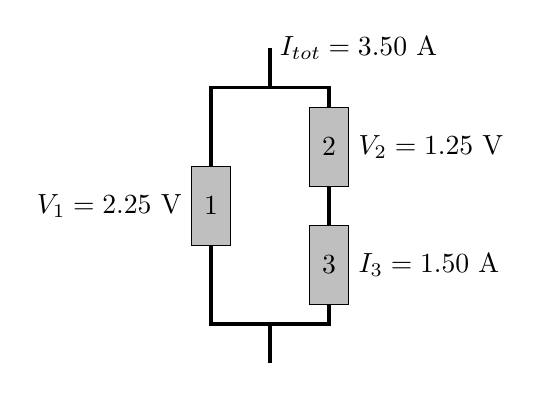
\begin{tikzpicture}

	% Circuit elements
	
	\begin{scope}[gray!50, draw = black]

		\filldraw (-1, -0.5) rectangle (-0.5, 0.5);
		\filldraw (1, 1.25) rectangle (0.5, 0.25);
		\filldraw (1, -1.25) rectangle (0.5, -0.25);
	
	\end{scope}
	
	\node at (-0.75, 0) {1};
	\node at (0.75, 0.75) {2};
	\node at (0.75, -0.75) {3};
	
	% Wires
	
	\begin{scope}[very thick]
		
		\draw (0, 1.5) -- (0, 2);
		\draw (-0.75, 0.5) -- (-0.75, 1.5) -- (0.75, 1.5) -- (0.75, 1.25);
		\draw (0.75, 0.25) -- (0.75, -0.25);
		\draw (-0.75, -0.5) -- (-0.75, -1.5) -- (0.75, -1.5) -- (0.75, -1.25);
		\draw (0, -1.5) -- (0, -2);
	
	\end{scope}
	
	% Given currents, voltages
	
	\node [right] at (0, 2) {$I_{tot} = 3.50$ A};
	\node [left] at (-1, 0) {$V_1 = 2.25$ V};
	\node [right] at (1, 0.75) {$V_2 = 1.25$ V};
	\node [right] at (1, -0.75) {$I_3 = 1.50$ A};

\end{tikzpicture}

\vspace{1em}

% INT_AY21_L30_Fig03_Missing_curr_volt.png

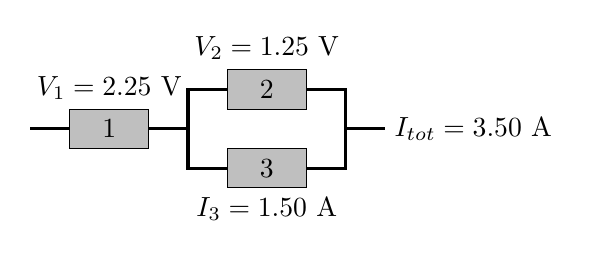
\begin{tikzpicture}

	% Circuit elements
	
	\begin{scope}[gray!50, draw = black]
	
		\filldraw (-1.5, -0.25) rectangle (-0.5, 0.25);
		\filldraw (0.5, 0.75) rectangle (1.5, 0.25);
		\filldraw (0.5, -0.75) rectangle (1.5, -0.25);
	
	\end{scope}
	
	\node at (-1, 0) {1};
	\node at (1, 0.5) {2};
	\node at (1, -0.5) {3};
	
	% Wires
	
	\begin{scope}[very thick]
		
		\draw (-1.5, 0) -- (-2, 0);
		\draw (-0.5, 0) -- (0, 0) -- (0, 0.5) -- (0.5, 0.5);
		\draw (0, 0) -- (0, -0.5) -- (0.5, -0.5);
		\draw (1.5, 0.5) -- (2, 0.5) -- (2, 0) -- (2.5, 0);
		\draw (1.5, -0.5) -- (2, -0.5) -- (2, 0);
	
	\end{scope}
	
	% Given currents, voltages
	
	\node [right] at (2.5, 0) {$I_{tot} = 3.50$ A};
	\node [above] at (-1, 0.25) {$V_1 = 2.25$ V};
	\node [above] at (1, 0.75) {$V_2 = 1.25$ V};
	\node [below] at (1, -0.75) {$I_3 = 1.50$ A};

\end{tikzpicture}

\vspace{1em}

% INT_AY20_L09_Fig01_I-V-graphs.png

\begin{tikzpicture}

	% Definition
	
	\def\L{1.5}
	
	% Matrix of graphs

	\matrix[column sep = 0.25 cm, ampersand replacement = \&]{
	
	\draw (0, \L) node [above] {$I$} -- (0, 0) -- (\L, 0) node [right] {$V$};
	\draw [red, thick] (0.1 * \L, 0.9 * \L) parabola [bend at end] (0.9 * \L, 0.1 * \L);
	\node [blue] at (0.5 * \L, -0.25 * \L) {$A.$};
	
	\&
	
	\draw (0, \L) node [above] {$I$} -- (0, 0) -- (\L, 0) node [right] {$V$};
	\draw [red, thick] (0, 0.8 * \L) -- (0.9 * \L, 0.8 *\L);
	\node [blue] at (0.5 * \L, -0.25 * \L) {$B.$};
	
	\&
	
	\draw (0, \L) node [above] {$I$} -- (0, 0) -- (\L, 0) node [right] {$V$};
	\draw [red, thick] (0, 0) parabola (0.9 * \L, 0.9 * \L);
	\node [blue] at (0.5 * \L, -0.25 * \L) {$C.$};
	
	\&
	
	\draw (0, \L) node [above] {$I$} -- (0, 0) -- (\L, 0) node [right] {$V$};
	\draw [red, thick] (0, 0) -- (0.9 * \L, 0.9 * \L);
	\node [blue] at (0.5 * \L, -0.25 * \L) {$D.$};
	
	\\
	};

\end{tikzpicture}

\vspace{1em}

% INT_AY20_L10_Fig01_Example_circuit.png

\begin{circuitikz}[voltage dir = old]

	\ctikzset { bipoles/length = 1 cm}
	
	\draw (0, 0) to [R, l = $R_1$] (0, 1.5) to [R, l = $R_2$] (0, 3) node [above] {$A$} to [short, *-*] (1.5, 3) node [above] {$B$}
		to [short, -*] (3, 3) node [above] {$C$} to [battery1, -*] (3, 1.5) node [right] {$E$} to [battery1, -*] (3, 0) node [below] {$H$}
		to [short, -*] (1.5, 0) node [below] {$G$} to [short, -*] (0, 0) node [below] {$F$}
		(3, 1.5) to [R, l = $R_4$, -*] (1.5, 1.5) node [left] {$D$}
		(1.5, 3) to [R, l_ = $R_3$, -*] (1.5, 1.5) to [R, l_ = $R_5$] (1.5, 0);

\end{circuitikz}

\vspace{1em}

% INT_AY20_L10_Fig02_Junction_rule.png

\begin{circuitikz}[voltage dir = old]

	% Circuit portion

	\draw [thick] (0, 0) to [short, -*] (1.5, 0) -- (1.5, 1.5)
		(1.5, 0) -- (4.5, 0) to [short, -*] (4.5, -1) -- (6, -1)
		(4.5, -1) -- (4.5, -2.5);
		
	% Current arrows
	
	\begin{scope}[->, > = latex, very thick, blue]
	
		\draw (1.65, 1.25) -- node [midway, right] {5.00 A} (1.65, 0.25);
		\draw (2.5, -0.15) -- node [midway, below] {8.00 A} (3.5, -0.15);
		\draw (4.35, -1.25) -- node [midway, left] {2.00 A} (4.35, -2.25);
		\draw (4.75, -0.85) -- node [midway, above] {$I = $ ?} (5.75, -0.85);
	
	\end{scope}

\end{circuitikz}

\vspace{1em}

% INT_AY21_L30_Fig03_Resistor_symbol.png

\begin{circuitikz}

	\ctikzset { bipoles/length = 1 cm}
	\draw (0, 0) to [R] (1.5, 0);

\end{circuitikz}

\vspace{1em}

% INT_AY21_L30_Fig04_Battery_symbol.png

\begin{circuitikz}

	\ctikzset { bipoles/length = 1 cm}
	\draw (0, 0) to [battery1] (1.5, 0);

\end{circuitikz}

\vspace{1em}

% INT_AY21_L30_Fig05_Simple_circuit.png

\begin{circuitikz}

	\ctikzset { bipoles/length = 1 cm}
	
	\draw (0, 0) to [R, l_ = $R$] (1.5, 0) -- (1.5, 1.5) to [battery1, l_ = {4.50 V}] (0, 1.5) -- (0, 0);
	
	\filldraw (0, 0) circle (1 pt) node [below left] {$A$};
	\filldraw (0, 1.5) circle (1 pt) node [above left] {$B$};
	\filldraw (1.5, 1.5) circle (1 pt) node [above right] {$C$};
	\filldraw (1.5, 0) circle (1 pt) node [below right] {$D$};

\end{circuitikz}

\vspace{1em}

% INT_AY21_L31_Fig01_Series_resistors.png

\begin{circuitikz}[> = latex]

	\ctikzset { bipoles/length = 1 cm}
	
	\draw (0, 0) to [R, l = $R_1$] (1.5, 0) to [R, l = $R_2$] (3, 0) to [R, l = $R_3$] (4.5, 0);
	
	\draw (6.5, 0) to [R, l = $R_{eq}$] (8, 0);
	
	\begin{scope}[->]
	
		\draw (0.25, -0.25) -- node [below] {$I_1$} (1.25, -0.25);
		\draw (1.75, -0.25) -- node [below] {$I_2$} (2.75, -0.25);
		\draw (3.25, -0.25) -- node [below] {$I_3$} (4.25, -0.25);
		
		\draw [thick] (5, 0) -- (6, 0);
		
		\draw (6.75, -0.25) -- node [below] {$I$} (7.75, -0.25);
	
	\end{scope}

\end{circuitikz}

\vspace{1em}

% INT_AY20_MP3_L12_Fig01_Series_circuit.png

\begin{circuitikz}

	\ctikzset { bipoles/length = 1 cm}

	\draw (0, 0) to [battery1, l = \mbox{$V = 90.0$ V}] (0, 2) to [resistor, l = \mbox{$R_1 = 10.0\ \Omega$}] (3, 2)
		to [resistor, l = \mbox{$R_2 = 15.0\ \Omega$}] (3, 0) to [resistor, l = \mbox{$R_3 = 20.0\ \Omega$}] (0, 0);

\end{circuitikz}

\vspace{1em}

% INT_AY20_MP3_L12_Fig02_Series_simplify.png

\begin{circuitikz}

	\ctikzset {bipoles/length = 1 cm}
	
	% Original circuit

	\draw (0, 0) to [battery1, l = \mbox{90.0 V}] (0, 2) to [resistor, l = \mbox{$R_1 = 10.0\ \Omega$}] (3, 2)
		to [resistor, l = \mbox{$R_2 = 15.0\ \Omega$}] (3, 0) to [resistor, l = \mbox{$R_3 = 20.0\ \Omega$}] (0, 0);
		
	% Arrow for simplification
	
	\draw [->, very thick, > = latex] (1.5, -0.75) -- (1.5, -1.25);
	
	% Simplified circuit
		
	\begin{scope}[yshift = -4 cm]

		\draw (0, 0) to [battery1, l = \mbox{90.0 V}] (0, 2) to [resistor, l = \mbox{$R_{123} = 45.0\ \Omega$}] (3, 2)
			-- (3, 0) -- (0, 0);
	
	\end{scope}

\end{circuitikz}

\vspace{1em}

% INT_AY20_MP3_L12_Fig03_Series_practice.png

\begin{circuitikz}

	\ctikzset { bipoles/length = 1 cm}

	\draw (0, 0) to [battery1, l = $V$] (0, 2) to [resistor, l = $R_1$] (3, 2)
		to [resistor, l = $R_2$] (3, 0) to [resistor, l = $R_3$] (0, 0);

\end{circuitikz}

\vspace{1em}

% INT_AY20_MP3_L12_Fig04_Parallel_example.png

\begin{circuitikz}[font = \scriptsize]

	\ctikzset { bipoles/length = 1 cm}
	
	% Actual circuit
	
	\draw (2, 0) -- (1, 0) to [battery1, l = \mbox{$V = 90.0$ V}] (1, 1.5) -- (2, 1.5)
		(4, 0) -- (2, 0) to [resistor, l_ = \mbox{$R_1 = 10.0\ \Omega$}] (2, 1.5) -- (4, 1.5)
		(6, 0) -- (4, 0) to [resistor, l_ = \mbox{$R_2 = 15.0\ \Omega$}] (4, 1.5) -- (6, 1.5)
			to [resistor, l = \mbox{$R_3 = 20.0\ \Omega$}] (6, 0);

\end{circuitikz}

\vspace{1em}

% INT_AY21_L31_Fig02_Parallel_resistors.png

\begin{circuitikz}[> = latex]

	\ctikzset { bipoles/length = 1 cm}
	
	\draw (0, 1) -- (0, 0.75);
	\draw (-1.5, 0.75) -- (1.5, 0.75);
	\draw (-1.5, -0.75) -- (1.5, -0.75);
	\draw (0, -0.75) -- (0, -1);
	
	\draw (-1.5, 0.75) to [R, l = $R_1$] (-1.5, -0.75);
	\draw (0, 0.75) to [R, l = $R_2$] (0, -0.75);
	\draw (1.5, 0.75) to [R, l = $R_3$] (1.5, -0.75);
	
	\draw (4.5, 1) to [R, l = $R_{eq}$] (4.5, -1);
	
	\begin{scope}[->]
	
		\draw (-1.75, 0.5) -- node [left] {$I_1$} (-1.75, -0.5);
		\draw (-0.25, 0.5) -- node [left] {$I_2$} (-0.25, -0.5);
		\draw (1.25, 0.5) -- node [left] {$I_3$} (1.25, -0.5);
		
		\draw [thick] (2.5, 0) -- (3.5, 0);
		
		\draw (4.25, 0.5) -- node [left] {$I$} (4.25, -0.5);
	
	\end{scope}

\end{circuitikz}

\vspace{1em}

% INT_AY20_MP3_L12_Fig05_Parallel_simplify.png

\begin{circuitikz}[font = \scriptsize]

	\ctikzset { bipoles/length = 1 cm}
	
	% Actual circuit
	
	\draw (2, 0) -- (1, 0) to [battery1, l = \mbox{$V = 90$ V}] (1, 1.5) -- (2, 1.5)
		(4, 0) -- (2, 0) to [resistor, l_ = \mbox{$R_1 = 10.0\ \Omega$}] (2, 1.5) -- (4, 1.5)
		(6, 0) -- (4, 0) to [resistor, l_ = \mbox{$R_2 = 15.0\ \Omega$}] (4, 1.5) -- (6, 1.5)
			to [resistor, l = \mbox{$R_3 = 20.0\ \Omega$}] (6, 0);
			
	% Arrow of simplification
	
	\draw [->, > = latex, very thick] (3.5, -0.125) -- (3.5, -0.625);
			
	% Simplified circuit
	
	\begin{scope}[xshift = 2.5 cm, yshift = -2.25 cm]
	
		\draw (2, 0) -- (0, 0) to [battery1, l = \mbox{$V = 90.0$ V}] (0, 1.5) -- (2, 1.5)
			to [resistor, l = \mbox{$R_{123} = 4.615\ \Omega$}] (2, 0);
		
	\end{scope}

\end{circuitikz}

\vspace{1em}

% INT_AY20_MP3_L12_Fig06_Parallel_practice.png

\begin{circuitikz}[font = \scriptsize]
	
	\ctikzset{bipoles/length = 1 cm}
	
	% Circuit A
	
	\draw (1, 0) -- (0, 0) to [battery1, l = $V$] (0, 1.5) -- (1, 1.5)
		(2, 0) -- (1, 0) to [resistor, l_ = $R_1$] (1, 1.5) -- (2, 1.5)
		(3, 0) -- (2, 0) to [resistor, l_ = $R_2$] (2, 1.5) -- (3, 1.5)
		(3, 0) to [resistor, l_ = $R_3$] (3, 1.5);
	
\end{circuitikz}

\vspace{1em}

% INT_AY20_MP3_L13_Fig01_Hybrid_example.png

\begin{circuitikz}

	% Front matter

	\def\d{1}
	\ctikzset{bipoles/length = \d cm}
	
	% Actual circuit
	
	\draw (0, 0) to [battery1, l = $V$] (0, 1.5 * \d)
		(0, 0) to [resistor, l = $R_2$] (-1.5 * \d, 0) to [resistor, l = $R_1$] (-1.5 * \d, 1.5 * \d) -- (0, 1.5 * \d)
		(0, 0) -- (1.5 * \d, 0) to [resistor, l_ = $R_4$] (1.5 * \d, 1.5 * \d) to [resistor, l_ = $R_3$] (0, 1.5 * \d);

\end{circuitikz}

\vspace{1em}

% INT_AY20_MP3_L13_Fig02_Hybrid_redraw.png

\begin{circuitikz}

	% Front matter

	\def\d{0.75}
	\ctikzset{bipoles/length = \d cm}
	
	\matrix[column sep = 0.25 cm]{
	
	% Actual circuit
	
	\begin{scope}[yshift = 0.5 cm]
	
	\draw (0, 0) to [battery1, l = $V$] (0, 1.5 * \d)
		(0, 0) to [resistor, l = $R_2$] (-1.5 * \d, 0) to [resistor, l = $R_1$] (-1.5 * \d, 1.5 * \d) -- (0, 1.5 * \d)
		(0, 0) -- (1.5 * \d, 0) to [resistor, l_ = $R_4$] (1.5 * \d, 1.5 * \d) to [resistor, l_ = $R_3$] (0, 1.5 * \d);
		
	\end{scope}
		
	&
	
	% Redrawing arrow
	
	\draw [<->, > = latex] (0, 1.5 * \d) -- (\d, 1.5 * \d);
	
	&
	
	% Redrawn circuit
	
	\draw (0, 0) -- (0, -0.25 * \d) -- (-2 * \d, -0.25 * \d) to [battery1, l = $V$] (-2 * \d, 3.25 * \d) -- (0, 3.25 * \d) -- (0, 3 * \d)
		(0, 0) -- (-\d, 0) to [resistor, l_ = $R_2$] (-\d, 1.5 * \d) to [resistor, l_ = $R_1$] (-\d, 3 * \d) -- (\d, 3 * \d)
		(\d, 3 * \d) to [resistor, l = $R_3$] (\d, 1.5 * \d) to [resistor, l = $R_4$] (\d, 0) -- (0, 0);
	
	\\	
	};

\end{circuitikz}

\vspace{1em}

% INT_AY20_MP3_L13_Fig03_First_redraw.png

\begin{circuitikz}

	% Front matter

	\def\d{0.75}
	\ctikzset{bipoles/length = \d cm}
	
	% Combine R1 and R2
	
	\draw (0, 0) -- (0, -0.25 * \d) -- (-2 * \d, -0.25 * \d) to [battery1, l = $V$] (-2 * \d, 3.25 * \d) -- (0, 3.25 * \d) -- (0, 3 * \d)
		(0, 0) -- (-\d, 0) to [resistor, l_ = $R_{12}$] (-\d, 3 * \d) -- (\d, 3 * \d)
		(\d, 3 * \d) to [resistor, l = $R_3$] (\d, 1.5 * \d) to [resistor, l = $R_4$] (\d, 0) -- (0, 0);

\end{circuitikz}

\vspace{1em}

% INT_AY20_MP3_L13_Fig04_Second_redraw.png

\begin{circuitikz}

	% Front matter

	\def\d{0.75}
	\ctikzset{bipoles/length = \d cm}
	
	% Combine R3 and R4
	
	\draw (0, 0) -- (0, -0.25 * \d) -- (-2 * \d, -0.25 * \d) to [battery1, l = $V$] (-2 * \d, 1.75 * \d) -- (0, 1.75 * \d) -- (0, 1.5 * \d)
		(0, 0) -- (-\d, 0) to [resistor, l_ = $R_{12}$] (-\d, 1.5 * \d) -- (\d, 1.5 * \d)
		(\d, 1.5 * \d) to [resistor, l = $R_{34}$] (\d, 0) -- (0, 0);

\end{circuitikz}

\vspace{1em}

% INT_AY20_MP3_L13_Fig05_Final_redraw.png

\begin{circuitikz}

	% Front matter

	\def\d{0.75}
	\ctikzset{bipoles/length = \d cm}
		
	% Combine R12 and R34
	
	\draw (0, 0) to [battery1, l = $V$] (0, 1.5 * \d) -- (2 * \d, 1.5 * \d) to [resistor, l = $R_{1234}$] (2 * \d, 0) -- (0, 0);

\end{circuitikz}

\vspace{1em}

% INT_AY21_L31_Fig03_Hybrid_practice.png

\begin{circuitikz}

	\ctikzset{bipoles/length = 0.75 cm}
	
	\draw (0, -1.5) to [R, l = $R_1$] (0, 0) -- (1.5, 0) to [battery1, l = $V$] (1.5, -3.25) -- (0, -3.25) -- (0, -3);
	\draw (-0.5, -1.5) -- (0.5, -1.5);
	\draw (-0.5, -1.5) to [R, l_ = $R_2$] (-0.5, -3);
	\draw (0.5, -1.5) to [R, l = $R_3$] (0.5, -3);
	\draw (-0.5, -3) -- (0.5, -3);

\end{circuitikz}

\vspace{1em}

% INT_AY21_L31_Fig04_Hybrid_practice.png

\begin{circuitikz}

	\ctikzset{bipoles/length = 0.75 cm}
	
	\draw (3, 0) to [battery1, l_ = $V$] (0, 0) to (0, 1) to [R, l = $R_G$] (1.5, 1) to [R, l = $R_J$] (3, 1) -- (3, -1) to [R, l = $R_H$] (0, -1) -- (0, 0);

\end{circuitikz}

\vspace{1em}

% INT_AY21_L32_Fig01_Wheatstone_bridge.png

\begin{circuitikz}

	\ctikzset{bipoles/length = 0.75 cm}
	
	\draw (-1, 0) to [R, l = $R_5$] (1, 0);
	\draw (-1, 0) to [R, l = $R_1$] (0, 1) to [R, l = $R_3$] (1, 0) to [R, l = $R_4$] (0, -1) to [R, l = $R_2$] (-1, 0);
	\draw (0, 1) -- (0, 1.5) -- (-2.5, 1.5) to [battery1, l = $V$] (-2.5, -1.5) -- (0, -1.5) -- (0, -1);
	
	\filldraw (-1, 0) circle (1 pt) node [left] {$A$};
	\filldraw (1, 0) circle (1 pt) node [right] {$B$};

\end{circuitikz}

\vspace{1em}

% INT_AY21_L32_Fig02_Circuit_w_real_batteries.png

\begin{circuitikz}

	\ctikzset{bipoles/length = 0.75 cm}
	
	\filldraw [gray!20] (0.25, 1.25) rectangle (2.75, 0.25);
	\filldraw [gray!20] (0.25, -1.75) rectangle (2.75, -0.625);
	
	\draw (3, 1) to [battery1, l = $V_1$] (1.5, 1) to [R, l = $R_1$] (0, 1) -- (0, 0) to [R, l_ = $R_3$] (3, 0);
	\draw (3, 1) -- (3, -1) to [battery1, l = $V_2$] (1.5, -1) to [R, l = $R_2$] (0, -1) -- (0, 0);

\end{circuitikz}

\vspace{1em}

% INT_AY20_MP3_L19_Fig01_Indep_eqns_example.png

\begin{circuitikz}

	\ctikzset { bipoles/length = 0.75 cm}
	
	% Actual circuit

	\draw (0, 0) to [R] (0, 3) -- (1.5, 3) node [above] {$A$} to [R, *-] (1.5, 1.5) to [R, -*] (1.5, 0) node [below] {$B$} to [battery1] (0, 0)
		(1.5, 0) to [battery1] (3, 0) to [R] (3, 3) -- (1.5, 3);
		
	% Current arrows and labels
	
	\begin{scope}[->, > = latex, very thick, blue]
	
		\draw (-0.375, 1) -- node [midway, left] {$I_1$} (-0.375, 2);
		\draw (3.375, 1) -- node [midway, right] {$I_2$} (3.375, 2);
		\draw (1.875, 2) -- node [midway, right] {$I_3$} (1.875, 1);
	
	\end{scope}

\end{circuitikz}

\vspace{1em}

% INT_AY20_MP3_L19_Fig02_Indep_eqns_example.png

\begin{circuitikz}

	\ctikzset { bipoles/length = 0.75 cm}
	
	% Actual circuit

	\draw (0, 0) to [R] (0, 3) -- (1.5, 3) node [above] {$D$} to [R, *-] (1.5, 1.5) to [R, -*] (1.5, 0) node [below] {$F$} to [battery1] (0, 0)
		(1.5, 0) to [battery1] (4, 0) to [R, -*] (4, 3) node [above right] {$E$} -- (1.5, 3)
		(1.5, 0) to [R] (4, 3);
		
	% Current arrows and labels
	
	\begin{scope}[->, > = latex, very thick, blue]
	
		\draw (-0.375, 1) -- node [midway, left] {$I_1$} (-0.375, 2);
		\draw (1.125, 1) -- node [midway, left] {$I_2$} (1.125, 2);
		\draw (2.25, 3.15) -- node [midway, above] {$I_3$} (3.25, 3.15);
		\draw (3.25, 1.5) -- node [midway, below right] {$I_4$} ++ ({180 + atan(3/2.5)} : 1);
		\draw (4.375, 2) -- node [midway, right] {$I_5$} (4.375, 1);
	
	\end{scope}

\end{circuitikz}

\vspace{1em}

% INT_AY20_MP3_L19_Fig03_Indep_eqns_practice.png

\begin{circuitikz}

	\ctikzset { bipoles/length = 1 cm}
	
	% Actual circuit
	
	\draw (0, 0) node [below left] {$A$} to [R, *-] (0, 3) to [R, -*] (3, 3) node [above] {$B$} to [R] (6, 3) to [battery1] (6, 1.5) to [R, *-] (3, 1.5)
		(0, 0) to [R] (3, 3) -- (3, 1.5) node [above left] {$D$} to [R, *-*] (3, 0) node [below] {$C$}
		(6, 1.5) node [above right] {$E$} -- (6, 0) to [R] (3, 0) to [battery1] (0, 0);
		
	% Circuit arrows and labels
	
	\begin{scope}[->, > = latex, very thick, blue]
	
		\draw [rounded corners] (-0.15, 2.5) -- (-0.15, 3.15) node [above left] {$I_1$} -- (0.5, 3.15);
		\draw (1, 1.5) -- node [midway, above left] {$I_2$} ++ (45 : 1);
		\draw (1, -0.5) -- node [midway, below] {$I_3$} (2, -0.5);
		\draw (4, 3.375) -- node [midway, above] {$I_4$} (5, 3.375);
		\draw (3.15, 1.75) -- node [midway, right] {$I_5$} (3.15, 2.75);
		\draw (2.625, 0.25) -- node [midway, left] {$I_6$} (2.625, 1.25);
		\draw (4, 1.875) -- node [midway, above] {$I_7$} (5, 1.875);
		\draw (6.15, 0.25) -- node [midway, right] {$I_8$} (6.15, 1.25);
	
	\end{scope}

\end{circuitikz}

\vspace{1em}

% INT_AY21_L32_Fig03_Intersecting_lines.png

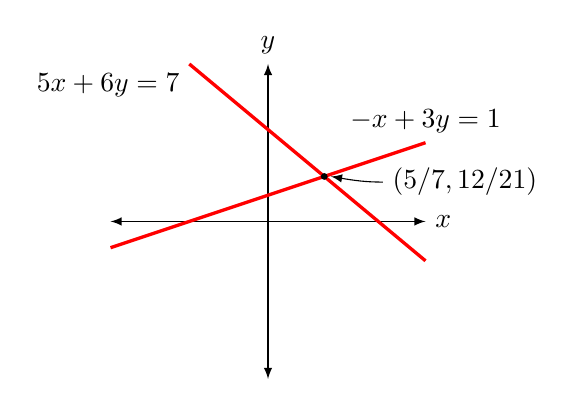
\begin{tikzpicture}[> = latex]

	% Axes
	
	\draw [<->] (-2, 0) -- (2, 0) node [right] {$x$};
	\draw [<->] (0, -2) -- (0, 2) node [above] {$y$};
	
	% Lines w/equations
	
	\begin{scope}[red, very thick]
	
		\draw (-1, 2) -- (2, -1/2);
		\draw (-2, -1/3) -- (2, 1);
		
	\end{scope}
	
	\node [below left] at (-1, 2) {$5x + 6y = 7$};
	\node [above] at (2, 1) {$-x + 3y = 1$};
	
	% Intersection point
	
	\filldraw (5/7, 12/21) circle (1 pt);
	\node (coords) at (2.5, 0.5) {$(5/7, 12/21)$};
	\draw [->] (coords.west) to [out = 180, in = -10] (0.8, 12/21);

\end{tikzpicture}

\vspace{1em}

% INT_AY20_MP3_L19_Fig04_Battery_volt_change.png

\begin{circuitikz}[> = latex]

	\ctikzset{bipoles/length = 1 cm}
	
	\matrix[column sep = 1.5 cm]{
	
	% Circuit element

	\draw (2, 0) node [right] {$B$} to [battery1, l_ = $V$, *-*] (0, 0) node [left] {$A$};
	
	% Equation for voltage change
	
	\node at (1, -0.75) {$\Delta V_{A \to B} = +V$};
	
	% Box
	
	\draw [gray, thin] (-0.5, -1) rectangle (2.5, 1);
	
	&
	
	% Circuit element

	\draw (0, 0) node [left] {$A$} to [battery1, l = $V$, *-*] (2, 0) node [right] {$B$};
	
	% Equation for voltage change
	
	\node at (1, -0.75) {$\Delta V_{A \to B} = -V$};
	
	% Box
	
	\draw [gray, thin] (-0.5, -1) rectangle (2.5, 1);
	
	\\
	};

\end{circuitikz}

\vspace{1em}

% INT_AY20_MP3_L19_Fig05_Resistor_volt_change.png

\begin{circuitikz}[> = latex]

	\ctikzset{bipoles/length = 1 cm}
	
	\matrix[column sep = 1.5 cm]{
	
	% Circuit element

	\draw (0, 0) node [left] {$A$} to [R, l = $R$, *-*] (2, 0) node [right] {$B$};
	
	% Arrow for current direction
	
	\draw [->, very thick, blue] (0.5, -0.375) -- node [midway, below] {$I$} (1.5, -0.375);
	
	% Equation for voltage change
	
	\node at (1, -1.25) {$\Delta V_{A \to B} = - IR$};
	
	% Box
	
	\draw [gray, thin] (-0.5, -1.5) rectangle (2.5, 0.625);
	
	&
	
	% Circuit element

	\draw (0, 0) node [left] {$A$} to [R, l = $R$, *-*] (2, 0) node [right] {$B$};
	
	% Arrow for current direction
	
	\draw [->, very thick, blue] (1.5, -0.375) -- node [midway, below] {$I$} (0.5, -0.375);
	
	% Equation for voltage change
	
	\node at (1, -1.25) {$\Delta V_{A \to B} = + IR$};
	
	% Box
	
	\draw [gray, thin] (-0.5, -1.5) rectangle (2.5, 0.625);
	
	\\
	};

\end{circuitikz}

\vspace{1em}

% INT_AY21_L32_Fig04_Example_circuit.png

\begin{circuitikz}

	\ctikzset { bipoles/length = 0.75 cm}
	
	% Actual circuit
	
	\draw (0, 0) node [left] {$A$} to [R, *-*, l = $R_3$] (2.5, 0) node [below] {$C$} to [battery1, -*, l = $V_1$] (5, 0) node [right] {$D$}
		-- (2.5, 2.5) node [above] {$B$} to [R, *-*, l_ = $R_1$] (0, 0) to [R, l_ = $R_4$] (2.5, -2.5) to [battery1, l_ = $V_2$] (5, 0)
		(2.5, 2.5) to [R, l = $R_2$] (2.5, 0);
		
	% Circuit arrows and labels
	
	\begin{scope}[->, > = latex, very thick, blue]

		\draw (1.125, 2.125) -- node [above left] {$I_1$} (0.375, 1.375);
		\draw (2.25, 1.75) -- node [left] {$I_2$} (2.25, 0.75);
		\draw (3.5, 2) -- node [above right] {$I_3$} (4.25, 1.25);
		\draw (0.75, -0.25) -- node [below] {$I_4$} (1.75, -0.25);
		\draw (4.25, -0.5) -- node [below] {$I_5$} (3.25, -0.5);
		\draw (0.375, -1.375) -- node [below left] {$I_6$}(1.125, -2.125);
	
	\end{scope}

\end{circuitikz}

\vspace{1em}

% INT_AY21_L32_Fig05_Example_circuit_w_labels.png

\begin{circuitikz}[american voltages]

	\ctikzset { bipoles/length = 0.75 cm}
	
	% Actual circuit
	
	\draw (0, 0) node [left] {$A$} to [R, *-*, v^> = $R_3$] (2.5, 0) node [below] {$C$} to [battery1, -*, v^> = $V_1$] (5, 0) node [right] {$D$}
		-- (2.5, 2.5) node [above] {$B$} to [R, *-*, v> = $R_1$] (0, 0) to [R, v_> = $R_4$] (2.5, -2.5) to [battery1, v_> = $V_2$] (5, 0)
		(2.5, 2.5) to [R, v^>= $R_2$] (2.5, 0);
		
	% Circuit arrows and labels
	
	\begin{scope}[->, > = latex, very thick, blue]

		\draw (1, 2.25) -- node [above left] {$I_1$} (0.25, 1.5);
		\draw (2.25, 1.75) -- node [left] {$I_2$} (2.25, 0.75);
		\draw (3.5, 2) -- node [above right] {$I_3$} (4.25, 1.25);
		\draw (0.75, -0.25) -- node [below] {$I_4$} (1.75, -0.25);
		\draw (4.25, -0.5) -- node [below] {$I_5$} (3.25, -0.5);
		\draw (0.25, -1.5) -- node [below left] {$I_6$}(1, -2.25);
		
	\end{scope}

\end{circuitikz}

\vspace{1em}

% INT_AY20_MP3_L20_Fig01_Kirchhoff_example.png

\begin{circuitikz}

	\ctikzset{bipoles/length = 1 cm}
	
	% Actual circuit

	\draw (2, 4) -- (0, 4) to [battery1, l_ = $V_1$] (0, 2) to [R, l_ = $R_1$] (0, 0) -- (2, 0)
		to [R, l = $R_2$] (2, 2) to [battery1, l = $V_2$] (2, 4)
		(2, 0) -- (4, 0) to [R, l_ = $R_3$] (4, 2) -- (4, 4) -- (2, 4);

\end{circuitikz}

\vspace{1em}

% INT_AY21_L32_Fig06_Example_circuit_w_arrows.png

\begin{circuitikz}

	\ctikzset{bipoles/length = 1 cm}
	
	% Actual circuit

	\draw (2, 4) -- (0, 4) to [battery1, l_ = $V_1$] (0, 2) to [R, l_ = $R_1$] (0, 0) -- (2, 0) node [below] {$B$}
		to [R, *-, l = $R_2$] (2, 2) to [battery1, -*, l = $V_2$] (2, 4) node [above] {$A$}
		(2, 0) -- (4, 0) to [R, l_ = $R_3$] (4, 2) -- (4, 4) -- (2, 4);
		
	% Current arrows
	
	\begin{scope}[> = latex, ->, thick, blue]
	
		\draw (0.25, 1.5) -- node [right] {$I_1$} (0.25, 2.5);
		\draw (2.25, 1.5) -- node [right] {$I_2$} (2.25, 2.5);
		\draw (3.75, 1.5) -- node [left] {$I_3$} (3.75, 2.5);
	
	\end{scope}
	
\end{circuitikz}

\vspace{1em}

% INT_AY21_L32_Fig07_Example_circuit_w_signs.png

\begin{circuitikz}[american voltages]

	\ctikzset{bipoles/length = 1 cm}
	
	% Actual circuit

	\draw (2, 4) -- (0, 4) to [battery1, v_> = $V_1$] (0, 2) to [R, v_< = $R_1$] (0, 0) -- (2, 0) node [below] {$B$}
		to [R, *-, v^> = $R_2$] (2, 2) to [battery1, -*, v^> = $V_2$] (2, 4) node [above] {$A$}
		(2, 0) -- (4, 0) to [R, v_> = $R_3$] (4, 2) -- (4, 4) -- (2, 4);
		
	% Current arrows
	
	\begin{scope}[> = latex, ->, thick, blue]
	
		\draw (0.25, 1.5) -- node [right] {$I_1$} (0.25, 2.5);
		\draw (2.25, 1.5) -- node [right] {$I_2$} (2.25, 2.5);
		\draw (3.75, 1.5) -- node [left] {$I_3$} (3.75, 2.5);
	
	\end{scope}

\end{circuitikz}

\vspace{1em}

% INT_AY21_L32_Fig08_Practice_circuit.png

\begin{circuitikz}

	\ctikzset{bipoles/length = 1 cm}

	\draw (0, 0) node [below left] {$C$} to [R, *-*, l = $R_3$] (2, 2) node [above right] {$B$} to [battery1, -*, l = $V_2$] (2, 0)
		node [below right] {$D$} to [R, l = $R_2$] (0, 0)
		(2, 2) to [battery1, -*, l_ = $V_1$] (0, 2) node [above left] {$A$} to [R, l_ = $R_1$] (0, 0);
		
\end{circuitikz}

\vspace{1em}

% INT_AY20_MP3_L17_Fig01_Uncharged_cap_circuit.png

\begin{circuitikz}

	\ctikzset{bipoles/length = 1 cm}
	
	% Actual circuit
	
	\draw (0, 0) to [battery1, l = $V$] (0, 2) -- (4, 2) to [R, l = $R$] (4, 0) -- (0, 0)
		(2, 0) to [C, l = $C$] (2, 2);
		
	% Current arrows
	
	\begin{scope}[very thick, blue, <-, > = latex]
	
		\draw [rounded corners] (-0.25, 1.5) -- (-0.25, 2.25) node [above left] {$I_{tot}$} -- (0.5, 2.25);
		\draw [rounded corners] (1.25, 2.25) -- (1.75, 2.25) node [above right] {$I_{tot}$} -- (1.75, 1.5);
		\draw [rounded corners] (1.75, 0.5) -- (1.75, -0.25) node [below right] {$I_{tot}$} -- (1.25, -0.25);
	
	\end{scope}
	
	% Time stamp
	
	\node at (8, 1) {$t = 0$};

\end{circuitikz}

\vspace{1em}

% INT_AY20_MP3_L17_Fig02_Charged_cap_circuit.png

\begin{circuitikz}

	\ctikzset{bipoles/length = 1 cm}
	
	% Actual circuit
	
	\draw (0, 0) to [battery1, l = $V$] (0, 2) -- (4, 2) to [R, l = $R$] (4, 0) -- (0, 0)
		(2, 0) to [C, l = $C$] (2, 2);
		
	% Current arrows
	
	\begin{scope}[very thick, blue, <-, > = latex]
	
		\draw [rounded corners] (-0.25, 1.5) -- (-0.25, 2.25) node [above left] {$I_{tot}$} -- (0.5, 2.25);
		\draw [rounded corners] (3.75, 2.25) -- (4.25, 2.25) node [above right] {$I_{tot}$} -- (4.25, 1.5);
		\draw [rounded corners] (4.25, 0.5) -- (4.25, -0.25) node [below right] {$I_{tot}$} -- (3.75, -0.25);
	
	\end{scope}
	
	% Time stamp
	
	\node at (8, 1) {$t \to \infty$};

\end{circuitikz}

\vspace{1em}

% INT_AY20_MP3_L17_Fig03_Charging_RC_circuit.png

\begin{circuitikz}

	\ctikzset{bipoles/length = 0.75 cm}
	
	\matrix[column sep = 1 cm]{

	% Open switch circuit
	
	\draw (0.25, 1) -- ++ (30: 0.5);
	\draw (0.75, 1) to [short, o-] (1, 1) to [R, l = $R$] (2, 1) to [C, l = $C$] (2, 0) -- (0, 0) to [battery1, l = $V$] (0, 1) to [short, -o] (0.25, 1);
	
	% Time label
	
	\node at (1, -0.5) {$t < 0$};
	
	&

	% Closed switch circuit
	
	\draw (0.25, 1) -- (0.75, 1) to [short, o-] (1, 1) to [R, l = $R$] (2, 1) to [C, l = $C$] (2, 0)
		-- (0, 0) to [battery1, l = $V$] (0, 1) to [short, -o] (0.25, 1);
		
	% Current arrow
	
	\draw [<-, > = latex, very thick, blue] (0, 1.25) -- node [midway, above] {$I$} (1, 1.25);
	
	% Time label
	
	\node at (1, -0.5) {$t \ge 0$};
	
	\\
	};

\end{circuitikz}

\vspace{1em}

% INT_AY20_MP3_L18_Fig01_Discharging_RC_circuit.png

\begin{circuitikz}

	\ctikzset{bipoles/length = 0.75 cm}
	
	\matrix[column sep = 1 cm]{

	% Open switch circuit
	
	\draw (0.25, 1) -- ++ (30: 0.5);
	\draw (0.75, 1) to [short, o-] (1, 1) to [R, l = $R$] (2, 1) to [C, l = $C$] (2, 0) -- (0, 0) -- (0, 1) to [short, -o] (0.25, 1);
	
	% Time label
	
	\node at (1, 2) {$t < 0$};
	
	&

	% Closed switch circuit
	
	\draw (0.25, 1) -- (0.75, 1) to [short, o-] (1, 1) to [R, l = $R$] (2, 1) to [C, l = $C$] (2, 0)
		-- (0, 0) --  (0, 1) to [short, -o] (0.25, 1);
		
	% Current arrow
	
	\draw [->, > = latex, very thick, blue] (1.75, -0.25) -- node [midway, below] {$I$} (0.75, -0.25);
	
	% Time label
	
	\node at (1, 2) {$t \ge 0$};
	
	\\
	};

\end{circuitikz}

\vspace{1em}

% INT_AY21_L33_Fig01_Parallel_capacitors.png

\begin{circuitikz}[> = latex]

	\ctikzset { bipoles/length = 1 cm}
	
	\draw (0, 1) -- (0, 0.75);
	\draw (-1.5, 0.75) -- (1.5, 0.75);
	\draw (-1.5, -0.75) -- (1.5, -0.75);
	\draw (0, -0.75) -- (0, -1);
	
	\draw (-1.5, 0.75) to [C, l = $C_1$] (-1.5, -0.75);
	\draw (0, 0.75) to [C, l = $C_2$] (0, -0.75);
	\draw (1.5, 0.75) to [C, l = $C_3$] (1.5, -0.75);
	
	\draw (4.5, 1) to [C, l = $C_{eq}$] (4.5, -1);
	
	\draw [->, thick] (2.75, 0) -- (3.75, 0);

\end{circuitikz}

\vspace{1em}

% INT_AY21_L33_Fig02_Series_capacitors.png

\begin{circuitikz}[> = latex]

	\ctikzset { bipoles/length = 1 cm}
	
	\draw (0, 0) to [C, l = $C_1$] (1.5, 0) to [C, l = $C_2$] (3, 0) to [C, l = $C_3$] (4.5, 0);
	
	\draw (6.5, 0) to [C, l = $C_{eq}$] (8, 0);
	
	\begin{scope}[->]
	
		\draw (-0.25, -0.25) -- node [below] {$I_1$} (0.25, -0.25);
		\draw (1.25, -0.25) -- node [below] {$I_2$} (1.75, -0.25);
		\draw (2.75, -0.25) -- node [below] {$I_3$} (3.25, -0.25);
		
		\draw [thick] (5, 0) -- (6, 0);
		
		\draw (6.25, -0.25) -- node [below] {$I$} (6.75, -0.25);
	
	\end{scope}

\end{circuitikz}

\vspace{1em}

% INT_AY20_MP3_L15_Fig01_Hybrid_example.png

\begin{circuitikz}

	% Front matter

	\def\d{1}
	\ctikzset{bipoles/length = \d cm}
	
	% Actual circuit
	
	\draw (0, 0) to [battery1, l = $V$] (0, 1.5 * \d)
		(0, 0) to [C, l = $C_2$] (-1.5 * \d, 0) to [C, l = $C_1$] (-1.5 * \d, 1.5 * \d) -- (0, 1.5 * \d)
		(0, 0) -- (1.5 * \d, 0) to [C, l_ = $C_4$] (1.5 * \d, 1.5 * \d) to [C, l_ = $C_3$] (0, 1.5 * \d);

\end{circuitikz}

\vspace{1em}

% INT_AY20_MP3_L15_Fig02_Hybrid_redraw.png

\begin{circuitikz}

	% Front matter

	\def\d{0.75}
	\ctikzset{bipoles/length = \d cm}
	
	\matrix[column sep = 0.25 cm]{
	
	% Actual circuit
	
	\begin{scope}[yshift = 0.5 cm]
	
	\draw (0, 0) to [battery1, l = $V$] (0, 1.5 * \d)
		(0, 0) to [C, l = $C_2$] (-1.5 * \d, 0) to [C, l = $C_1$] (-1.5 * \d, 1.5 * \d) -- (0, 1.5 * \d)
		(0, 0) -- (1.5 * \d, 0) to [C, l_ = $C_4$] (1.5 * \d, 1.5 * \d) to [C, l_ = $C_3$] (0, 1.5 * \d);
		
	\end{scope}
		
	&
	
	% Redrawing arrow
	
	\draw [<->, > = latex] (0, 1.5 * \d) -- (\d, 1.5 * \d);
	
	&
	
	% Redrawn circuit
	
	\draw (0, 0) -- (0, -0.25 * \d) -- (-2 * \d, -0.25 * \d) to [battery1, l = $V$] (-2 * \d, 3.25 * \d) -- (0, 3.25 * \d) -- (0, 3 * \d)
		(0, 0) -- (-\d, 0) to [C, l_ = $C_2$] (-\d, 1.5 * \d) to [C, l_ = $C_1$] (-\d, 3 * \d) -- (\d, 3 * \d)
		(\d, 3 * \d) to [C, l = $C_3$] (\d, 1.5 * \d) to [C, l = $C_4$] (\d, 0) -- (0, 0);
	
	\\	
	};

\end{circuitikz}

\vspace{1em}

% INT_AY20_MP3_L15_Fig03_First_redraw.png

\begin{circuitikz}

	% Front matter

	\def\d{0.75}
	\ctikzset{bipoles/length = \d cm}
	
	% Combine C1 and C2
	
	\draw (0, 0) -- (0, -0.25 * \d) -- (-2 * \d, -0.25 * \d) to [battery1, l = $V$] (-2 * \d, 3.25 * \d) -- (0, 3.25 * \d) -- (0, 3 * \d)
		(0, 0) -- (-\d, 0) to [C, l_ = $C_{12}$] (-\d, 3 * \d) -- (\d, 3 * \d)
		(\d, 3 * \d) to [C, l = $C_3$] (\d, 1.5 * \d) to [C, l = $C_4$] (\d, 0) -- (0, 0);

\end{circuitikz}

\vspace{1em}

% INT_AY20_MP3_L15_Fig04_Second_redraw.png

\begin{circuitikz}

	% Front matter

	\def\d{0.75}
	\ctikzset{bipoles/length = \d cm}
	
	% Combine C3 and C4
	
	\draw (0, 0) -- (0, -0.25 * \d) -- (-2 * \d, -0.25 * \d) to [battery1, l = $V$] (-2 * \d, 1.75 * \d) -- (0, 1.75 * \d) -- (0, 1.5 * \d)
		(0, 0) -- (-\d, 0) to [C, l_ = $C_{12}$] (-\d, 1.5 * \d) -- (\d, 1.5 * \d)
		(\d, 1.5 * \d) to [C, l = $C_{34}$] (\d, 0) -- (0, 0);

\end{circuitikz}

\vspace{1em}

% INT_AY20_MP3_L15_Fig05_Final_redraw.png

\begin{circuitikz}

	% Front matter

	\def\d{0.75}
	\ctikzset{bipoles/length = \d cm}
		
	% Combine C12 and C34
	
	\draw (0, 0) to [battery1, l = $V$] (0, 1.5 * \d) -- (2 * \d, 1.5 * \d) to [C, l = $C_{1234}$] (2 * \d, 0) -- (0, 0);

\end{circuitikz}

\vspace{1em}

% INT_AY21_L33_Fig03_Hybrid_practice.png

\begin{circuitikz}

	\ctikzset{bipoles/length = 0.75 cm}
	
	\draw (0, -1.5) to [C, l = $C_1$] (0, 0) -- (1.5, 0) to [battery1, l = $V$] (1.5, -3.25) -- (0, -3.25) -- (0, -3);
	\draw (-0.5, -1.5) -- (0.5, -1.5);
	\draw (-0.5, -1.5) to [C, l_ = $C_2$] (-0.5, -3);
	\draw (0.5, -1.5) to [C, l = $C_3$] (0.5, -3);
	\draw (-0.5, -3) -- (0.5, -3);

\end{circuitikz}

\vspace{1em}

% INT_AY21_L33_Fig04_Hybrid_practice.png

\begin{circuitikz}

	\ctikzset{bipoles/length = 0.75 cm}
	
	\draw (3, 0) to [battery1, l_ = $V$] (0, 0) to (0, 1) to [C, l = $C_K$] (1.5, 1) to [C, l = $C_L$] (3, 1) -- (3, -1) to [C, l = $C_M$] (0, -1) -- (0, 0);

\end{circuitikz}

% INT_AY20_MP3_L17_Fig04_Exponential_graphs.png

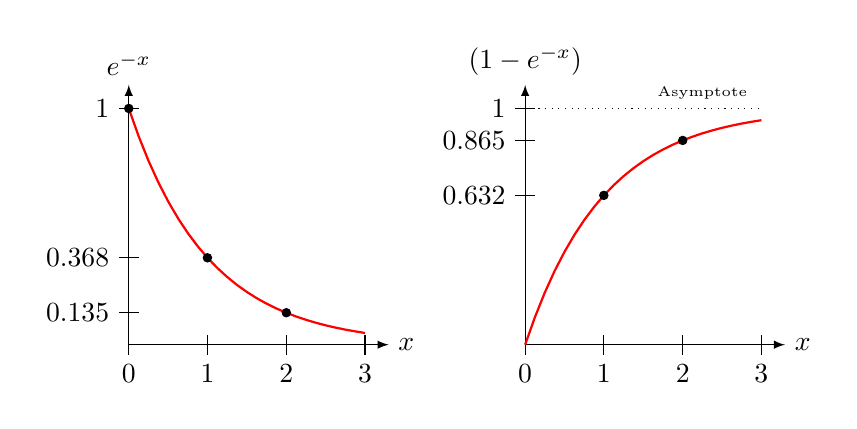
\begin{tikzpicture}

	% Definitions
	
	\def\X{3}	% Horizontal distance scale
	\def\Y{3}	% Vertical distance scale
	
	\matrix[column sep = 0.125 cm]{

	% Axes
	
	\draw [<->, > = latex] (0, 1.1 * \Y) node [above] {$e^{-x}$} -- (0, 0) -- (1.1 * \X, 0) node [right] {$x$};
	
	% Actual graph
	
	\draw [thick, red] plot[variable = \r, domain = 0:\X] (\r, {\Y * exp(-3 * \r / \X)});
	
	% Mark points on graph line
	
	\filldraw (0, \Y) circle (1.5 pt);
	\filldraw (0.333 * \X, {\Y * exp(-1)}) circle (1.5 pt);
	\filldraw (0.667 * \X, {\Y * exp(-2)}) circle (1.5 pt);
	
	% Marks on axes
	
	\draw (-0.125, \Y) node [left] {1} -- (0.125, \Y);
	\draw (-0.125, {\Y * exp(-1)}) node [left] {0.368} -- (0.125, {\Y * exp(-1)});
	\draw (-0.125, {\Y * exp(-2)}) node [left] {0.135} -- (0.125, {\Y * exp(-2)});
	
	\draw (0, 0) -- (0, -0.125) node [below] {0};
	\draw (0.333 * \X, 0.125) -- (0.333 * \X, -0.125) node [below] {1};
	\draw (0.667 * \X, 0.125) -- (0.667 * \X, -0.125) node [below] {2};
	\draw (\X, 0.125) -- (\X, -0.125) node [below] {3};

	&

	% Axes
	
	\draw [<->, > = latex] (0, 1.1 * \Y) node [above] {$(1 - e^{-x})$} -- (0, 0) -- (1.1 * \X, 0) node [right] {$x$};
	
	% Actual graph
	
	\draw [thick, red] plot[variable = \r, domain = 0:\X] (\r, {\Y * (1 - exp(-3 * \r / \X) )});
	
	% Mark points on graph line + asymptote
	
	\filldraw (0.333 * \X, {\Y * (1 -  exp(-1) )}) circle (1.5 pt);
	\filldraw (0.667 * \X, {\Y * (1 - exp(-2) )}) circle (1.5 pt);
	\draw [dotted] (0, \Y) -- node [near end, above, font = \tiny] {Asymptote} (\X, \Y);
	
	% Marks on axes
	
	\draw (-0.125, \Y) node [left] {1} -- (0.125, \Y);
	\draw (-0.125, {\Y * (1 - exp(-1) )}) node [left] {0.632} -- (0.125, {\Y * (1 - exp(-1) )});
	\draw (-0.125, {\Y * (1 - exp(-2) )}) node [left] {0.865} -- (0.125, {\Y * (1 - exp(-2) )});
	
	\draw (0, 0) -- (0, -0.125) node [below] {0};
	\draw (0.333 * \X, 0.125) -- (0.333 * \X, -0.125) node [below] {1};
	\draw (0.667 * \X, 0.125) -- (0.667 * \X, -0.125) node [below] {2};
	\draw (\X, 0.125) -- (\X, -0.125) node [below] {3};
	
	\\
	};

\end{tikzpicture}

\vspace{1em}

% INT_AY21_L33_Fig05_Capacitor_symbol.png

\begin{circuitikz}

	\ctikzset{bipoles/length = 1 cm}
	
	\draw (0, 0) to [C] (1, 0);

\end{circuitikz}

\vspace{1em}

% INT_AY21_L33_Fig06_Q_vs_V_graph.png

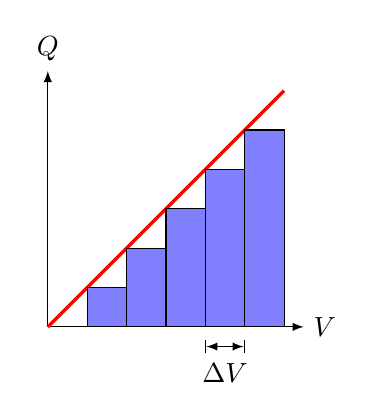
\begin{tikzpicture}[> = latex]

	% Axes
	
	\draw [<->] (0, 3.25) node [above] {$Q$} -- (0, 0) -- (3.25, 0) node [right] {$V$};
	
	% Graph curve
	
	\draw [very thick, red] (0, 0) -- (3, 3);
	
	% Rectangles
	
	\foreach \x in {0.5, 1, ..., 2.5}
		\filldraw [blue!50, draw = black] (\x, 0) rectangle ({\x + 0.5}, \x);
		
	\draw [|<->|] (2, -0.25) -- node [below = 0.25 em] {$\Delta V$} (2.5, -0.25);

\end{tikzpicture}

\end{document}